\documentclass[11pt, norsk]{article}
%\usepackage[latin1]{inputenc}
\usepackage[T1]{fontenc}
\usepackage[utf8]{inputenc}
\usepackage[norsk]{babel}   % S P R A A K
%%
%% husk 
%% git pull origin 
%% git add *
%% git commit -m "..."
%% git push
% \usepackage{graphicx}    % postscript graphics
\usepackage{amssymb, amsmath, amsthm, amssymb} % symboler, osv
\usepackage{mathrsfs,calligra}
\usepackage{url}
\usepackage{thmtools}
\usepackage{enumerate}  % lister $
\usepackage{float}
\usepackage{tikz}
\usepackage[all]{xy}   % for comm.diagram
\usepackage{wrapfig} % for float right
\usepackage[colorlinks=true]{hyperref} 
\usepackage{mystyle} % stilfilen      

\newtheorem{conj}{Formodning} 
\title{Notater speilsymmetry}
\author{Fredrik Meyer}
\date{}
\begin{document}
\maketitle

\section{Litt historie}

Kort historisk oppsummering.
\begin{itemize}
\item \textbf{1980s:} Studier av superstringkompaktifisering. ``Speilsymmetri''-prinsippet (og masse matematisk hurlumhei) sier at det burde eksistere to ``speil'', $X$ og $Y$ med lignende, men speilede egenskaper.
\item \textbf{1991:} Candelas, de la Ossa, Green Parkes: kom med formodning som spådde ``antall'' rasjonale kurver av alle grader på en grad 5 Calabi-Yau-mangfoldighet, uttrykt ved ``periodene'' til en holomorf 3-form på en annen ``speil''-mangfoldighet. 
\item \textbf{1994:} Maxim Kontsevich (han siste i ``Colors of Math''), foreslår en teori, ``homologisk speil-symmetri''. Formodningen er at det er en ekvivalens mellom to deriverte kategorier, hver assosiert til en Calabi-Yau-mangfoldighet. 
\item \textbf{1994:} Batyrev og Borisov viser hvordan en kan bruke torisk geometri for å konstruere eksempler på Calabi-Yau-mangfoldigheter. 
\item \textbf{1995:} Ellingsrud og Strømme viste at antall vridde kubikker på en generell kvintikk er {317.206.375}, noe som stemmer med det speilsymmetri forutsier.
\item \textbf{1996:} Stroming, Yau, Zaslow kom med sin ``SYZ-formodning''. Denne er veldig ``topologisk'', og inneholder ord som ``Lagrangian fibration'', ``torus bundles'', osv.
\item \textbf{1997:} Kreuzer og Skarke klassifiserte alle $4$-dimensjonale refleksive polytoper. Det er 473.800.776 av dem.
\item \textbf{2003:} Mark Gross, Berndt Siebert publiserte artikkelen ``Mirror Symmetry via Logarithmic Degeneration Data'' (144 sider!). Det er en algebraisk-geometrisk versjon av SYZ-formodningen. De bruker ideer som $\log$ geometri, tropisk geometri, polyhedre, torisk geometri, deformasjonsteori, nilpotente elementer, osv. Dette er hva Nordfjordeid skal gi en innføring i.
\end{itemize}

\section{Hva sier speilsymmetri?}

\subsection{Fysikk}

Noe om supersymmetrisk strengteori og egenvektorer. Valg av basis fører til valg av Calabi-Yau-mangfoldighet, men dette skal ikke ha noe å si. Resultat: to familier av Calabi-Yau.

Resten er hokus-pokus.


\subsection{Matematiske påstander}

Har ``noe å gjøre'' med Calabi-Yau-mangfoldigheter. Så la oss starte med definisjonen. 

\begin{defi}
  En Calabi-Yau mangfoldighet (av dimensjon $3$) er en glatt, proper varietet $X$ over $\C$ slik at den kanoniske bunten $\omega_X$ er triviell og slik at $H^j(X, \OO_X)=0$ for $j \neq 0,3$. 
\end{defi}

Husk at den kanoniske bunten er per definisjon $\bigwedge^n \Omega_X^1$. Lokalt er seksjoner av denne beskrevet som $f\, \d x_1 \wedge \d x_2 \wedge \cdots \wedge \d x_n$ for $f \in \OO_X(U)$. At den er triviell betyr at $\omega_X \simeq \OO_X$. Det finnes med andre ord en $n$-form $\omega \in \omega_X$ som aldri er null.

Det er andre definisjoner av Calabi-Yau, men de bruker ord jeg ikke kan (for å droppe ord: en kompakt $3$-dimensjonal kompleks mangfoldighet med en Kähler-metrikk $g$ slik at holonomi-gruppen er $SU(3)$). 

Til glatte komplekse mangfoldigheter kan vi tilordne \emph{Hodge-tall}. Disse er per definisjon $h^{ij}:= \dim_\C H^i(X,\Omega^j_X)$. Ved Serre-dualitet og kompleks konjugering følger det at $h^{ij}=h^{ji}$, så disse tallene er symmetriske. Fra dette, og betingelsen kan vi skrive opp ``Hodge-diamanten'':

\begin{verbatim}
             1
         0      0
     0      h^11    0  
  1    h^21      h12   1
     0      h^22   0   
         0      0
             1
\end{verbatim}

Hvor $h^{11}=h^{22}$ og $h^{12}=h^{21}$. Da er Euler-karakteristikken $\chi = 2(h^{11}-h^{12})$.

\begin{figure}
  \centering
    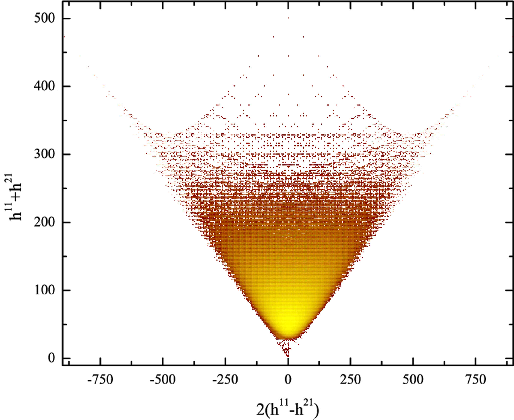
\includegraphics[width=0.5\textwidth]{hodgeplot.png}
  \caption{Hodge-plot av alle kjente Calabi-Yau-mangfoldigheter. }
\end{figure}

Nå kan vi komme  med én av speilsymmetriens formodninger:

\begin{conj}
 For hver Calabi-Yau $3$-mangfoldighet $X$, finnes en Calabi-Yau $3$-mangfoldighet $Y$ slik $h^{11}(X)=h^{21}(Y)$ og $h^{21}(X)=h^{11}(Y)$.
\end{conj}

Mer presist/vagt (alt etter som), sier påstanden at det finnes en dualitet mellom \emph{familier} av Calabi-Yau-mangfoldigheter. Enda mer ``presist'', skal variasjon av kompleks struktur på $X$ svare til variasjon av ``symplektisk struktur'' på $Y$ (hva nå enn det betyr!).

\subsection{Det kanoniske eksemplet: kvintikken}

La $X$ være en generell kvintikk i $\PP^4$, altså definert ved et generelt femtegradspolynom.

\begin{thm}
 $X$ er Calabi-Yau.
\end{thm}
\begin{proof}
De fleste varieteter er glatte, så $X$ er glatt. Projektive varieteter er propre. For å se at $h^1=h^2=0$, må man ty til teoremer. La $\II_X$ være idealknippet til $X$ i $\PP^4$. Men $\II_X \simeq \OO_{\PP^4}(-5)$, og $H^2(\OO_{\PP^4}(-5))=0$ ved et teorem i Hartshorne. Samme oppskrift for $H^2(\OO_X)$.

Alternativt: $X$ degenererer til et Stanley-Reisner-skjema med ideal $I=\langle x_0x_1\cdots x_4 \rangle$ som svarer til $\partial \Delta^4$, altså randen til en $4$-ball, som er en $3$-sfære. Et folketeorem i Stanley-Reisner-teori sier at $H^i(X,\OO_X) \simeq H^i(\mathcal K,\C)$ (der høyresiden er simplisialkohomologi). Så $X$ har kohomologien til en sfære.

For å vise at den kanoniske er triviell, har vi adjunksjonsteoremet (også fra Hartshorne), som sier at $K_X = \restr{(K_{\PP^4} + D_X) }{X}$. Klassen til $K_{\PP^4}$ er $5H$, der $H$ er klassen til et hyperplan. Her er $D_X=-5H$. Det følger at $K_X=\restr{5H-5H}{X}=0$, så $K_X$ er triviell.
\end{proof}

Neste spørsmål i utforskingen av $X$ er å regne ut Hodge-diamanten. For det trenger vi to tall: $h^{11}=\dim_\C H^1(X,\Omega^1_X)$ og $h^{12}=\dim_\C H^1(X, \Omega^2_X)$.

For å gjøre trenger man snitteori (eller mer erfaring). Svaret er at $h^{11}=1$ og $h^{12}=101$. Heuristisk dukker tallet $101$ opp på følgende måte: dimension $h^{12}$ skal svare til rommet av kvintiske hyperflater. Antall kvintikker opp til $\C^\ast$ $125$, men vi må trekke fra automorfier av $\PP^5$, som det er $24$ av. Så $h^{12}=101$. (ikke spør meg hvorfor!) \verb|Macaulay2| gir ihvertfall samme svar, med kommandoen \verb|HH^1(cotangentSheaf(2,X))|.

\subsubsection{Speilet til $X$}

Først av alt, $X$ passer naturlig inn i en familie $X_\psi$ av skjema, nesten alle Calabi-Yau:
\[
X_\psi = \{ x_0^5+x_1^5+x_2^5+x_3^5+x_4^5+\psi x_0x_1x_2x_3x_4x_5=0 \}
\]

Legg merke til at $X_\psi$ er invariant under den naturlige virkningen fra $(\Z_5)^5/\Z_5$. Undergruppen $H \subset G$ definert ved $\vec a \in H \Leftrightarrow \sum \vec a_i \equiv 0 \pmod 5$ virker på $X_\psi$, og det kan bli vist at kvotienten $X_\psi/H$ har en desingularisering som fortsatt er Calabi-Yau, og at denne har speilede Hodge-tall.

\section{Batyrev-Borisov-konstruksjonen}

BB-konstruksjonen er den sålangt mest fruktbare konstruksjonen av konkrete eksempler på Calabi-Yau-mangfoldigheter. Vi trenger noen begreper. Husk at et \emph{gitterpolytop} er et polytop med hjørner i et gitter $\Z^d$. 

\begin{defi}
Et gitter-polytop $\Delta$ er \emph{refleksivt} om det kun har ett indre gitterpunkt, og også $\Delta^\circ$ er et gitterpolytop. 
\end{defi}

Enkelt $2$-dimensjonalt eksempel: $\qed$ og $\diamond$. I tre dimensjoner er kuben og oktaederet polare. Det er bare endelig mange refleksive polytoper i en gitt dimensjon. 

La nå $\PP_\Delta$ være den toriske varieteten assosiert til polytopet $\Delta$. Dette kan bli realisert som $\Proj$ av $\C[\Z \cap C(\Delta \times \{ 1 \})]$, der $C(\Delta \times \{ 1 \})$ er kjeglen over polytopet. 

Her er Batyrev-Borisov-konstruksjonen: La $f$ være polynomet med monomer parametrisert av hjørnene til Newton-polytopet $\Delta$. Da er tillukningen til $Z(f)$ i $\PP_\Delta$ en Calabi-Yau-mangfoldighet.

Speilet er konstruert ved å gjøre det samme med det polare polytopet.

Denne konstruksjonen kan generaliseres til komplette snitt i mange dimensjoner.

\section{Gross-Siebert-programmet}

Toriske degenerasjoner.

Log geometri.

Lagrangian subvarieties? 




\end{document}
